% Very simple template for lab reports. Most common packages are already included.
\documentclass[a4paper, 11pt]{article}
\usepackage[utf8]{inputenc} % Change according to your file encoding
\usepackage{graphicx}
\usepackage{url}
\usepackage{listings}
\usepackage[table]{xcolor}
\usepackage{float} % provides [H] placement to pin floats
\usepackage{placeins} % provides \FloatBarrier to prevent floats from passing barriers
\usepackage{booktabs} % for professional-looking tables
\usepackage{titlesec} % for customizing section headings
\usepackage{subcaption} % for subfigures

% Customize section spacing for better visual separation
\titlespacing*{\section}{0pt}{12pt plus 4pt minus 2pt}{8pt plus 2pt minus 2pt}
\titlespacing*{\subsection}{0pt}{10pt plus 4pt minus 2pt}{6pt plus 2pt minus 2pt}
\titlespacing*{\subsubsection}{0pt}{8pt plus 4pt minus 2pt}{4pt plus 2pt minus 2pt}

%opening
\title{Report 4: IK2221 LLM inference project}
\author{Group 9: Riccardo Fragale, insert names}
\date{\today{}}

\begin{document}

\maketitle


\section{Task 1}
\subsection{Question 1: Latency vs. Sequence Length}
\subsubsection*{Evaluation methodology}
We decided to evaluate the impact of the sequence length on the prefill time (and in particular to the TTFT) with varying KV cache size (ranging from 0 to 4.0).
We recorded TTFT for every request and the combined sequence length of the context of the question and the length of the prompt.
The expectation is that TFFT grows sort of quadratically as the sequence length increases.
Due to a cold start of the model we also saw that the first request arriving was particularly slow (ruining all metrics and averages), while the next ones have a similar pattern
even though they involve a context switch. That's why we will show below some graphs regarding TTFT vs sequence length both including and not including the first request in order
to better show what we found out.
The benchmark provided (that could be added with --increasing-length ) includes ten random questions about the different contexts, done in a way such that they have an increasing sequence length.
This happens because the questions are selected inside three difference batches of prompts of different size.
The first batch includes some short and general prompts while the other ones include medium size and large size prompts.

\subsubsection*{Results and analysis}
 In order not to avoid a list of 15 graphs we decide to include here the ones we believe are more meaningful but you can explore all the logs and all the graphs of our tests inside the folders
  \path{lmcache-vllm-extended\docker\results\q1} and also the \path{lmcache-vllm-extended\docker\results\q1_polished}. The polished ones include the graphs without 
 the first request that, as said in the previous paragraph, ruins all averages and metrics and we haven't figured out why it is particularly slow.
 Let's first see what happens with cache size = 0 (so the model is not caching KV chunks actually).

\begin{figure}[H]
    \centering
    \begin{subfigure}{0.48\textwidth}
        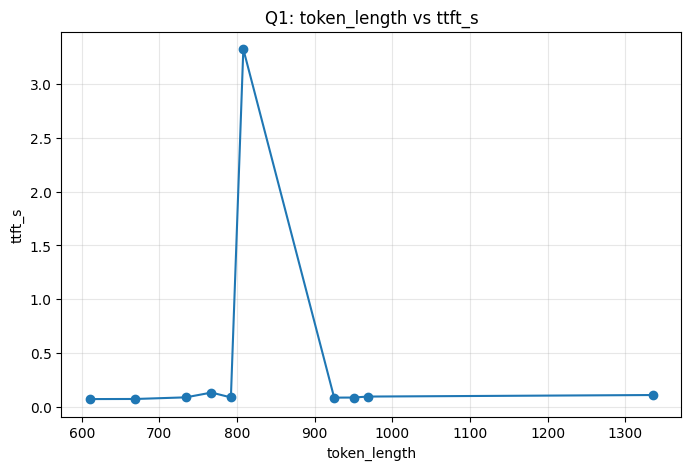
\includegraphics[width=\linewidth]{lmcache-vllm-extended/frontend/results/q1/graph_q1_0size.png}
        \caption{Normal logs (q1)}
    \end{subfigure}\hfill
    \begin{subfigure}{0.48\textwidth}
        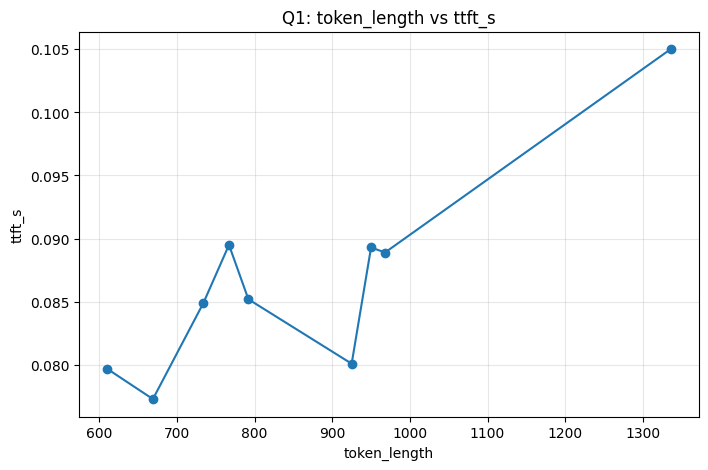
\includegraphics[width=\linewidth]{lmcache-vllm-extended/frontend/results/q1_polished/graph_q1_0size.png}
        \caption{Polished logs (q1\_polished)}
    \end{subfigure}
    \caption{TTFT vs. sequence length for cache size = GB}
    \label{fig:q1_cache0}
\end{figure}

The reason why we polished is the following:
\\
\noindent\textbf{Average TTFT:} 0.4146\,s.
\\
\textbf{Average TTFT excluding first request:} 0.0913\,s.
\\
Analysing the polished graph it's clear that there is a trend that seems quite quadratic, which is what we expected.
\\
Let's go now to cache size = 1.0 GB.
\begin{figure}[H]
    \centering
    \begin{subfigure}{0.48\textwidth}
        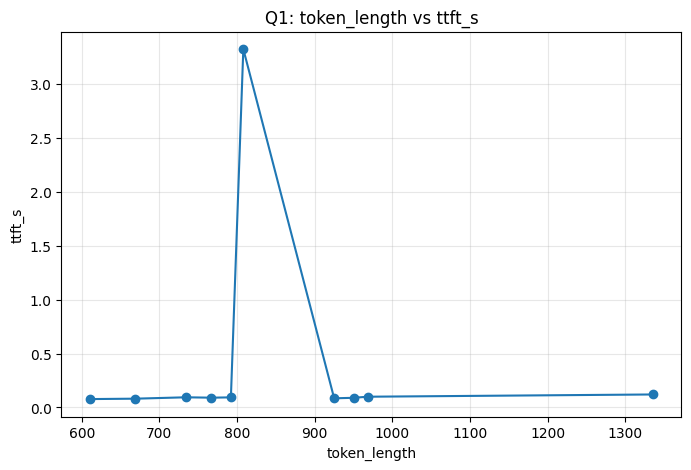
\includegraphics[width=\linewidth]{lmcache-vllm-extended/frontend/results/q1/graph_q1_10size.png}
        \caption{Normal logs (q1)}
    \end{subfigure}\hfill
    \begin{subfigure}{0.48\textwidth}
        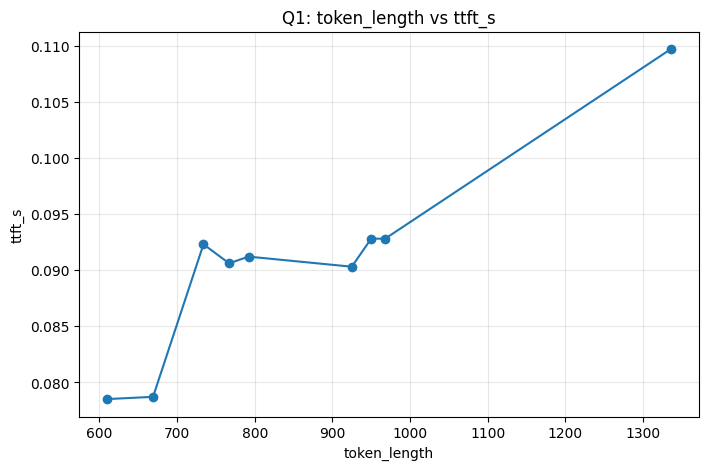
\includegraphics[width=\linewidth]{lmcache-vllm-extended/frontend/results/q1_polished/graph_q1_10size.png}
        \caption{Polished logs (q1\_polished)}
    \end{subfigure}
    \caption{TTFT vs. sequence length for cache size = 1 GB}
    \label{fig:q1_cache10}
\end{figure}

\noindent\textbf{Average TTFT:} 0.4156\,s.
\\
\textbf{Average TTFT excluding first request:} 0.0927\,s.
\\
\\
There is again a linear to quadratic trend. Increasing the cache didn't generate a noticeable improvement in TTFT.

Finally let's try to increase the cache size to 4 GB.
\begin{figure}[H]
    \centering
    \begin{subfigure}{0.48\textwidth}
        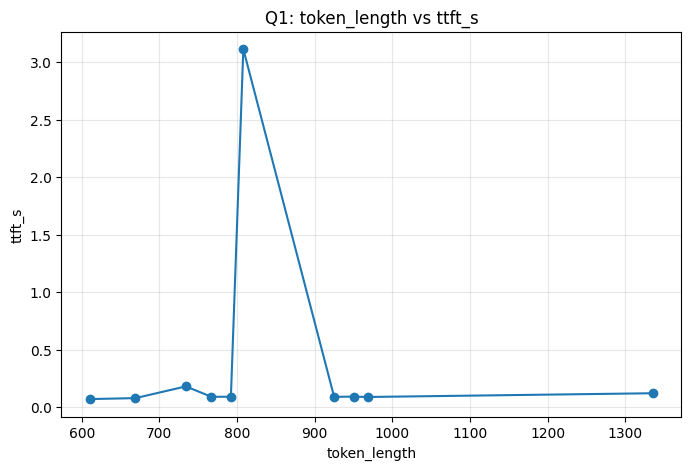
\includegraphics[width=\linewidth]{lmcache-vllm-extended/frontend/results/q1/graph_q1_40size.png}
        \caption{Normal logs (q1)}
    \end{subfigure}\hfill
    \begin{subfigure}{0.48\textwidth}
        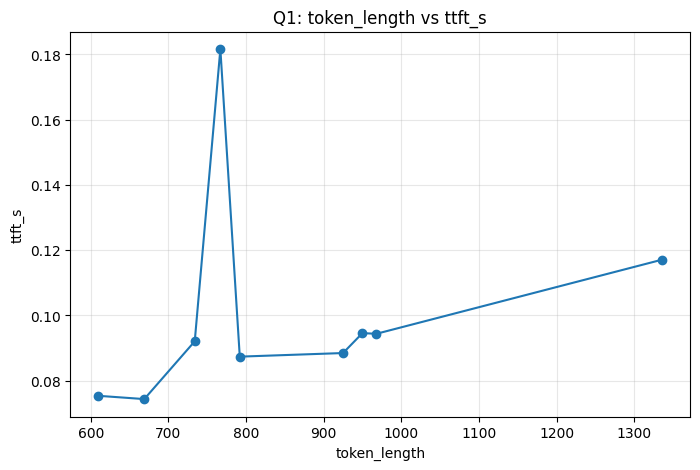
\includegraphics[width=\linewidth]{lmcache-vllm-extended/frontend/results/q1_polished/graph_q1_40size.png}
        \caption{Polished logs (q1\_polished)}
    \end{subfigure}
    \caption{TTFT vs. sequence length for cache size = 4 GB}
    \label{fig:q1_cache10}
\end{figure}

\noindent\textbf{Average TTFT:} 0.4017\,s.
\\
\textbf{Average TTFT excluding first request:} 0.1004\,s.
\\

In this case we also notice that a request was particularly "slow" in the prefill despite it's not so long in terms 
of size of context and prompt. This indicates that maybe sometimes during a context switch some operations is 
randomly particularly slow. 

To do a final summary, we have seen that the trend is quadratical (as expected) in almost each cache size as the impact of caching is not particularly relevant
to reduce TTFT considering the sequence length. We expect to be meaningful regarding the next questions since it is more helpful with
repeated requests about the same context as the KV remains in the GPu that is running the model.



 
 


\subsection{Question 2: KV Cache Reuse and Cache Size Impact}
\subsubsection*{Evaluation Methodology}
To rigorously evaluate the latency improvements and cache sensitivity, we configured the LMCache-extended backend with varying levels of \texttt{max\_local\_cache\_size} (ranging from 0.001 to 3.0). This parameter directly restricts or expands the available KV cache capacity. We then used a custom request generator running in a repeated sequence mode, querying the model with specific document contexts and repeating different questions within the same context before switching to a completely new context. 

We recorded the Time To First Token (TTFT) for every request. By plotting the sequence of requests, we can visually identify cache misses (when a new context is loaded, requiring full prompt evaluation) and cache hits (when a new question is asked for a previously cached context). We calculated the average TTFT for hits and misses across each configuration to observe caching effectiveness.

\subsubsection*{Results and Analysis}
As shown in our timeline visualizations (Figure~\ref{fig:q2_timelines}), feeding an old request to the model significantly reduces latency, provided the cache is large enough. The TTFT for cache hits (green markers) drops noticeably compared to cache misses (red markers), confirming that reusing the KV cache heavily optimizes inference time.

Furthermore, we analyzed how the size of the local cache affects these results. When the local cache size is extremely small (e.g., utilization = 0.001), the cache is unable to retain previously seen requests. This results in frequent evictions, causing identical latencies for both hits and misses, as the system is forced into recomputation. 

As the cache size increases (e.g., utilization $\ge$ 0.4), the system successfully stores the KV pairs. The gap between hit latency and miss latency widens significantly, showcasing the effectiveness of an adequately sized local cache. This overall trend is aggregated and clearly visible in Figure~\ref{fig:q2_summary}.

\begin{figure}[H]
    \centering
    \begin{subfigure}{0.48\textwidth}
        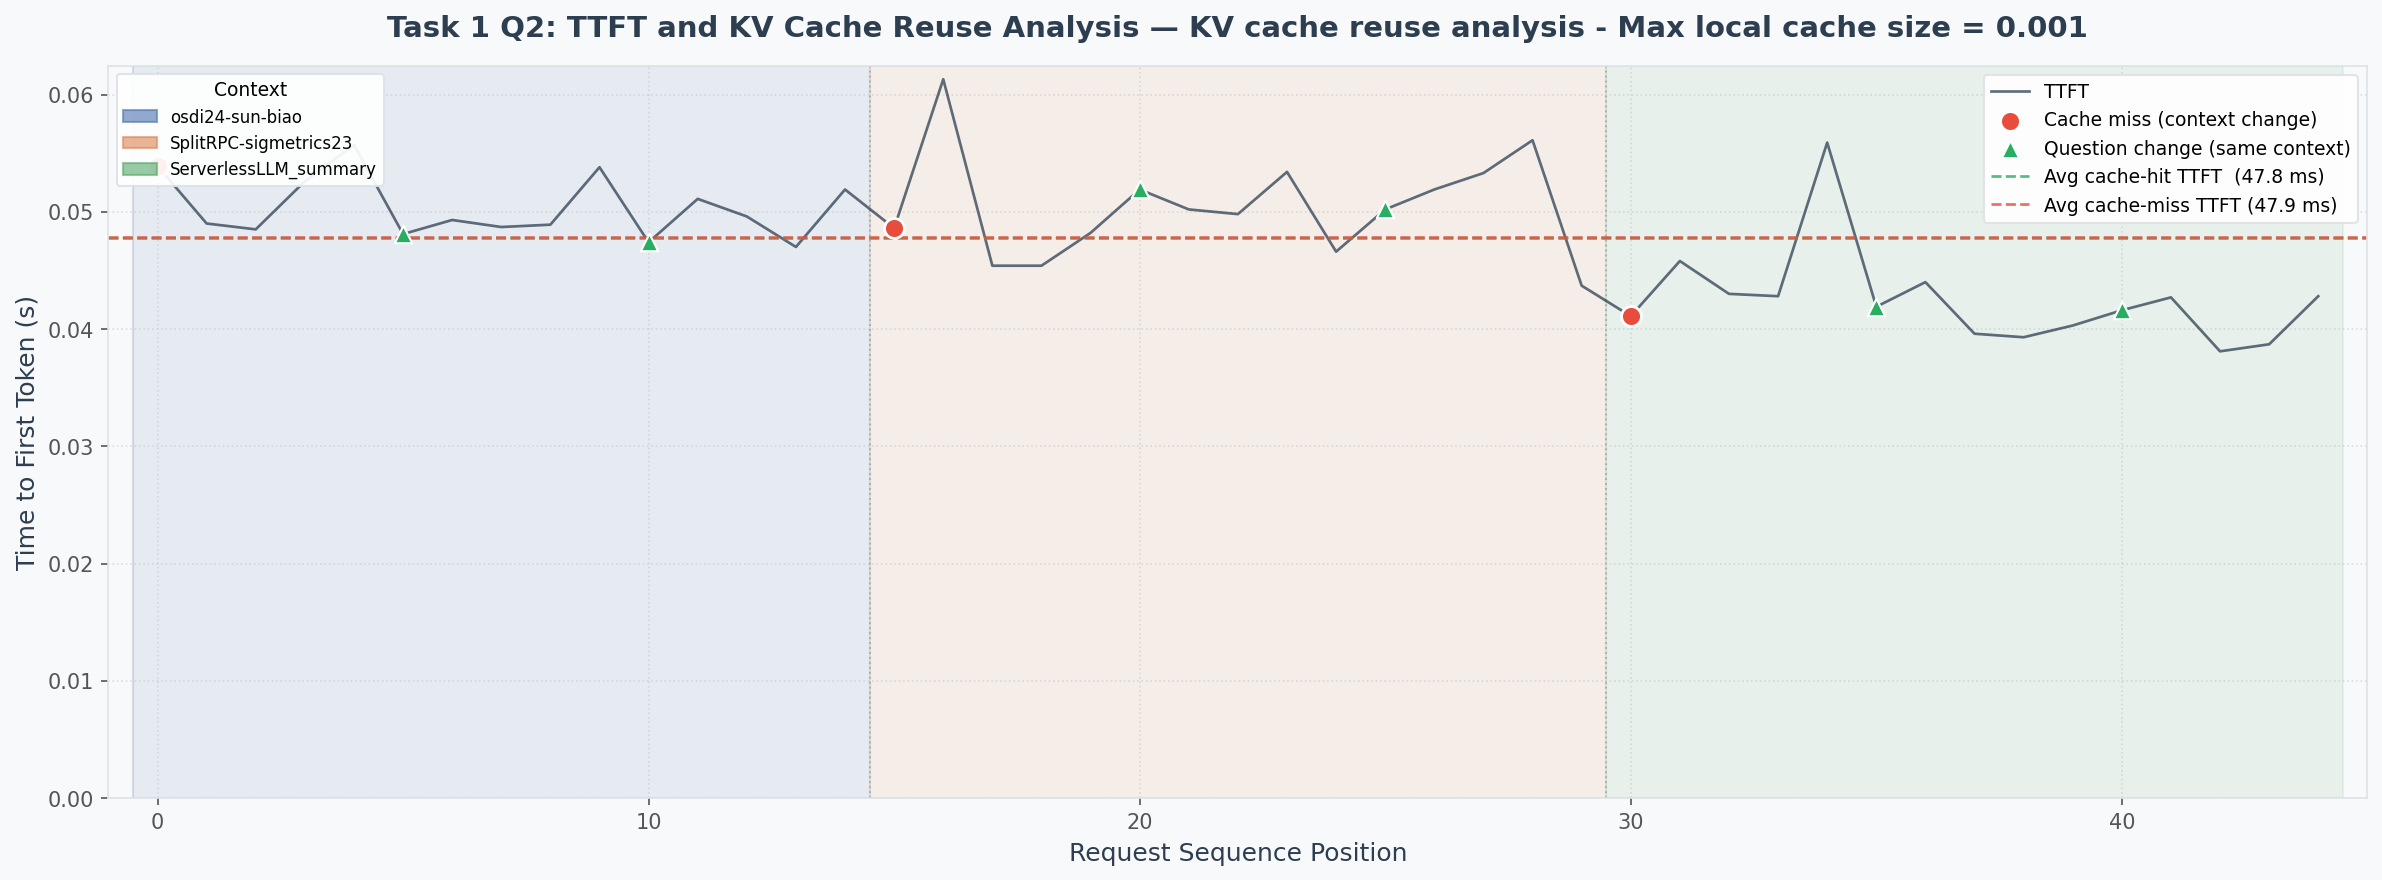
\includegraphics[width=\linewidth]{lmcache-vllm-extended/frontend/results/q2_new/q2_util_0.001.png}
        \caption{Util = 0.001 (Frequent Evictions)}
    \end{subfigure}\hfill
    \begin{subfigure}{0.48\textwidth}
        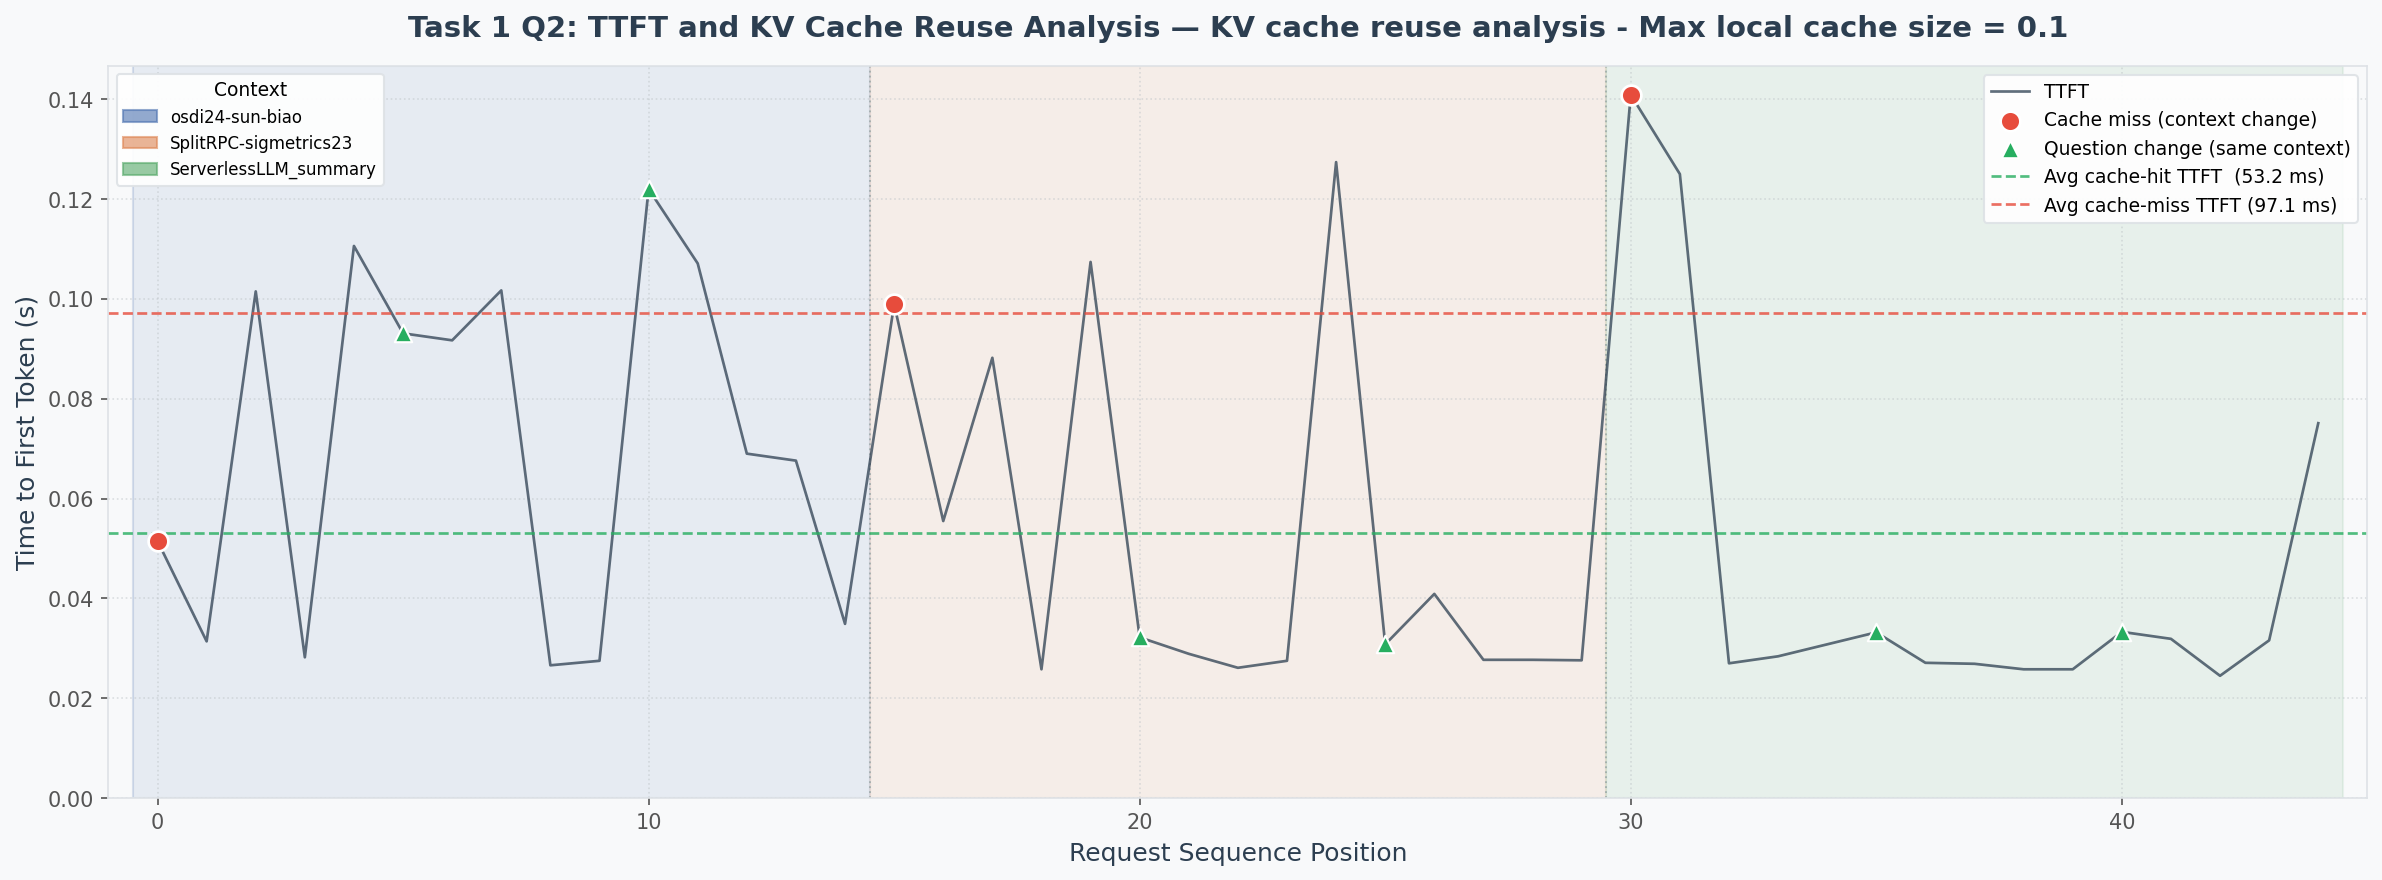
\includegraphics[width=\linewidth]{lmcache-vllm-extended/frontend/results/q2_new/q2_util_0.1.png}
        \caption{Util = 0.1 (Partial Caching)}
    \end{subfigure}
    
    \vspace{0.3cm}
    \begin{subfigure}{0.48\textwidth}
        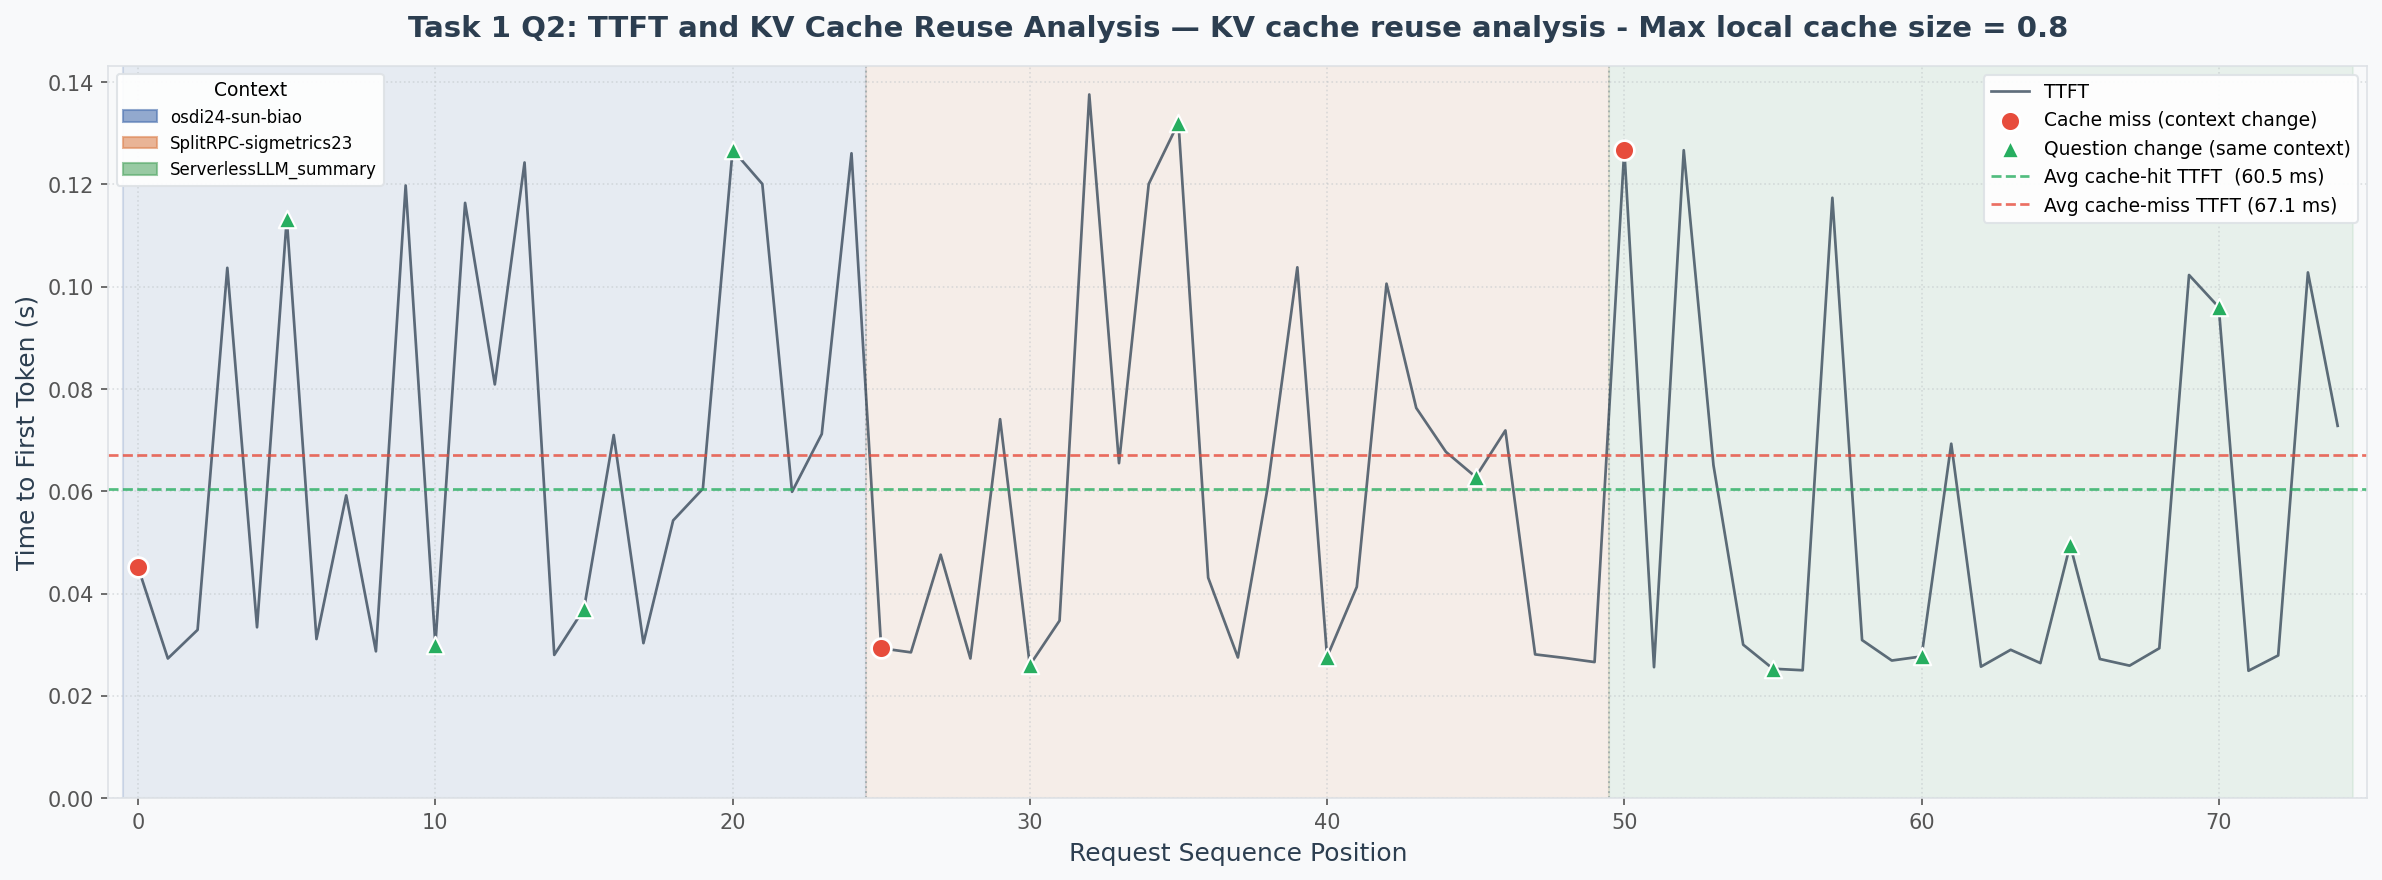
\includegraphics[width=\linewidth]{lmcache-vllm-extended/frontend/results/q2_new/q2_util_0.8.png}
        \caption{Util = 0.8 (Stable Caching)}
    \end{subfigure}\hfill
    \begin{subfigure}{0.48\textwidth}
        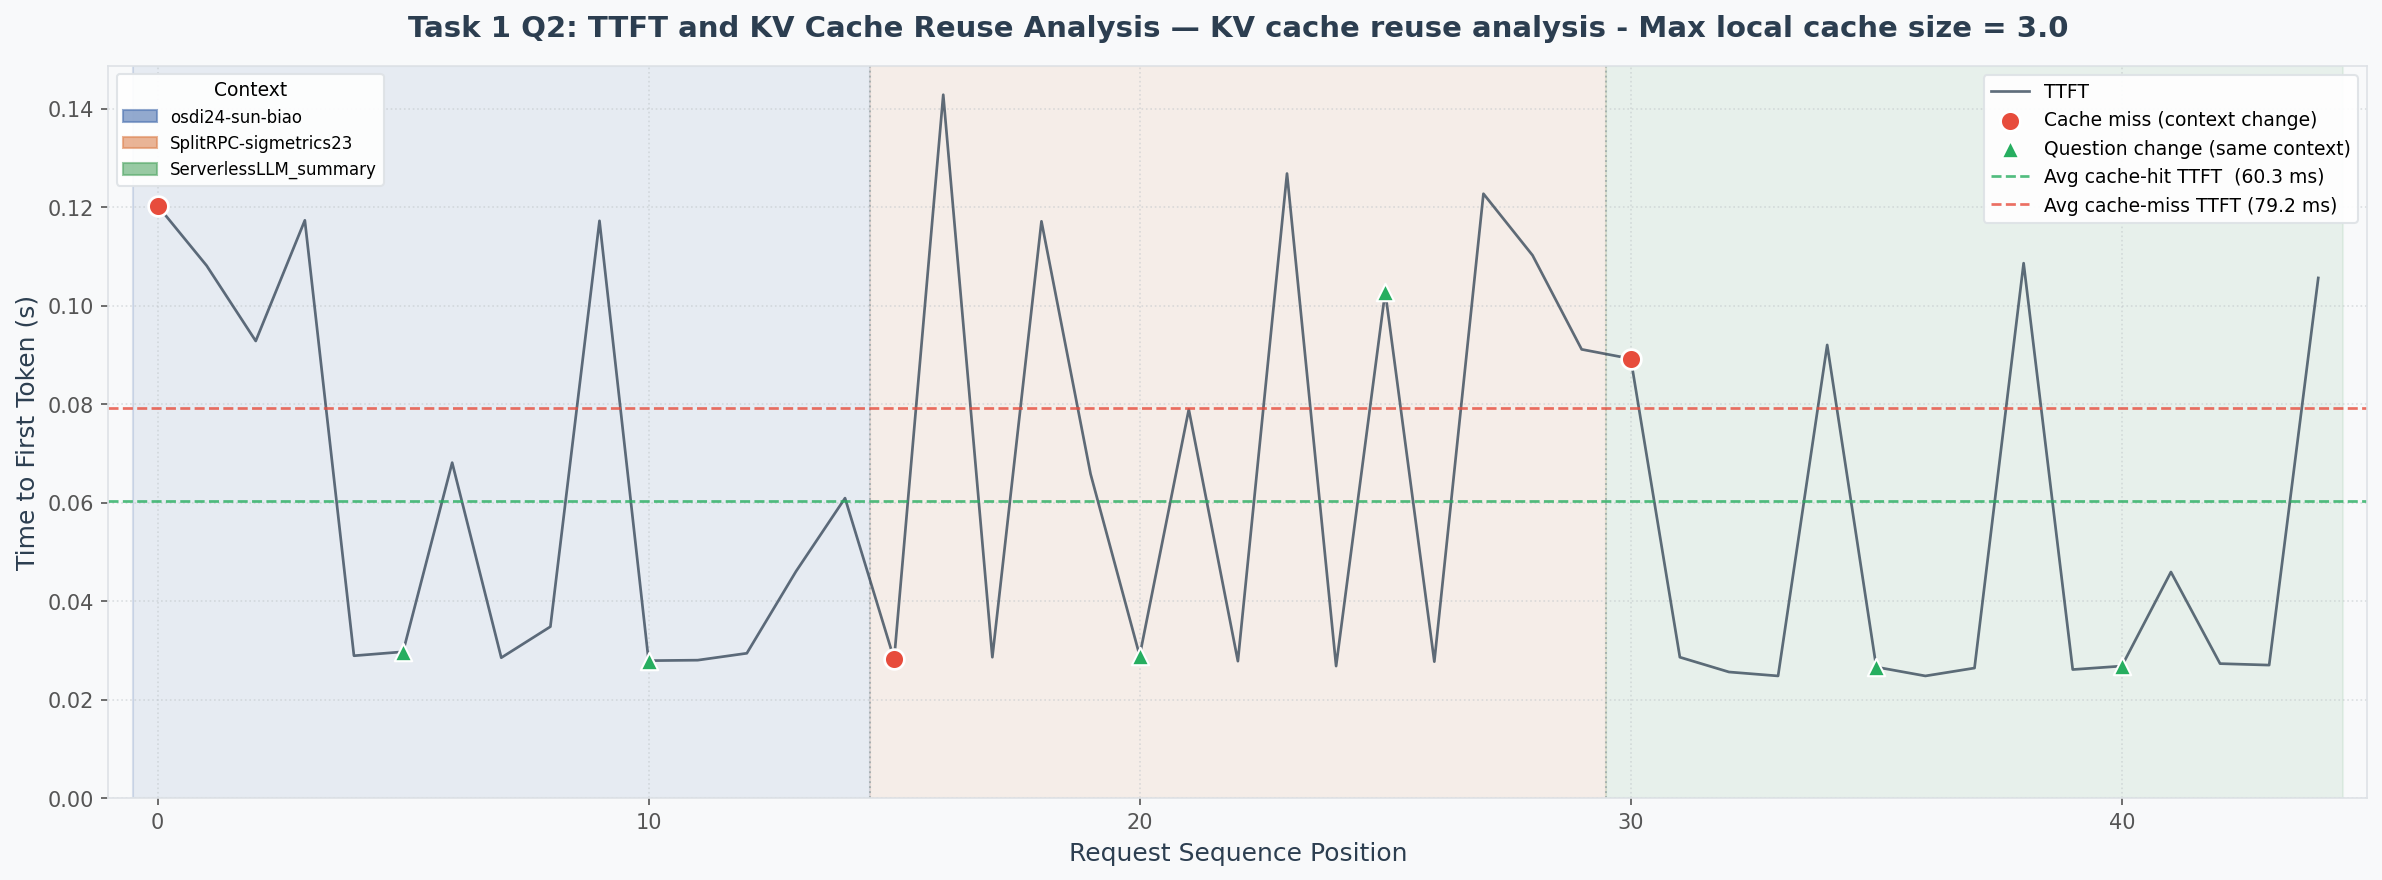
\includegraphics[width=\linewidth]{lmcache-vllm-extended/frontend/results/q2_new/q2_util_3.0.png}
        \caption{Util = 3.0 (Oversized Cache)}
    \end{subfigure}
    \caption{Timeline visualizations of TTFT across varying GPU KV cache size. At extremely low utilization, the cache size is insufficient, causing hit and miss latencies to converge. At higher utilizations, cache hits show distinctly lower TTFT.}
    \label{fig:q2_timelines}
\end{figure}

\begin{figure}[H]
    \centering
    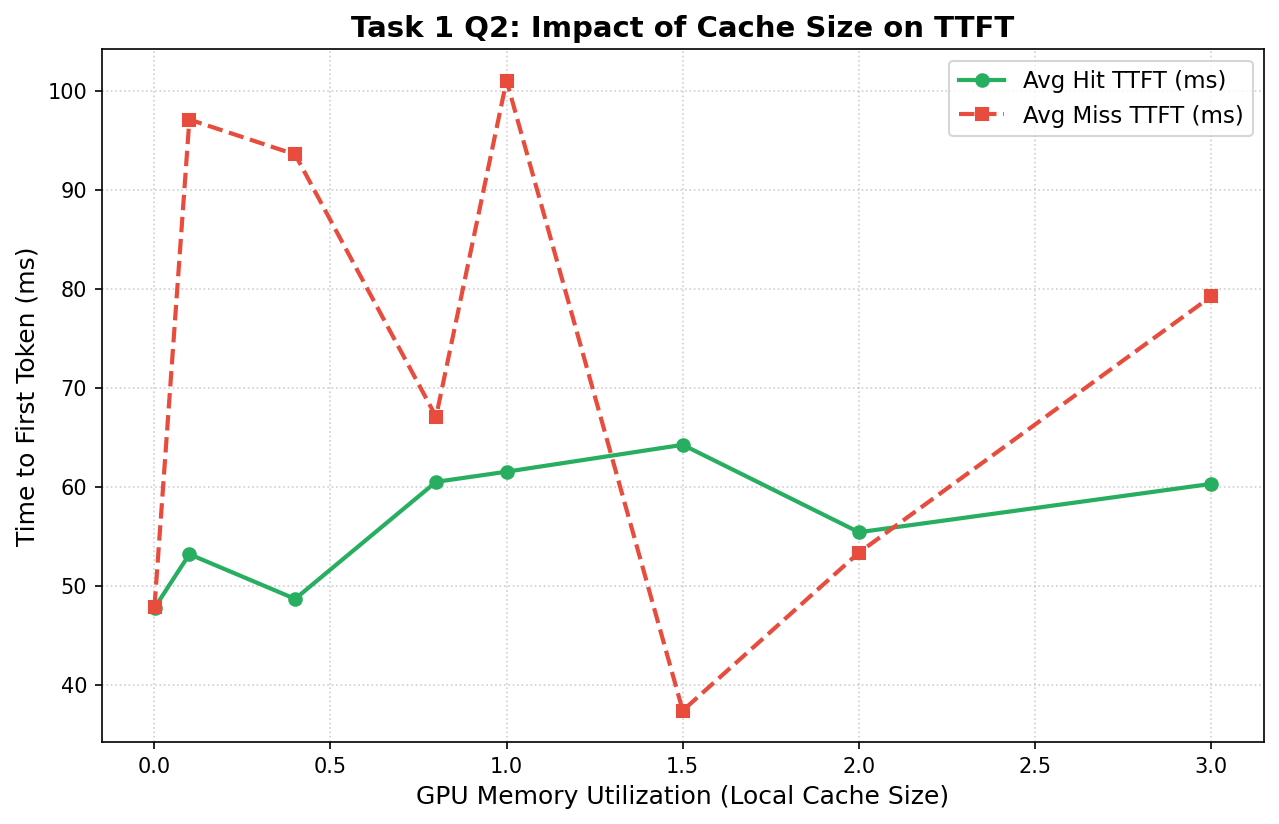
\includegraphics[width=0.8\textwidth]{lmcache-vllm-extended/frontend/results/q2_new_summary.png}
    \caption{Impact of KV cache size on Average TTFT. The gap between misses and hits demonstrates caching efficiency.}
    \label{fig:q2_summary}
\end{figure}

\subsection{Question 3: Impact of Request Diversity}

\subsubsection*{Testing setup}
For evaluating the impact of request/context diversity on system performance, we used the same custom request generator but on a random mode. The random mode creates the request list by iterating through the context list, creating a new request with a random question from the question list at each iteration, until the specified number of requests is reached. This request list is then served sequentially to the LLM. In this manner, we are able to feed the LLM with a diverse set of requests, without repetition of contexts in sequential requests. This test setup allows us to see how the system performs under increased request and order diversity. We also introduce a random-extended test mode, which forms requests on a larger context set, so we can see how increasing the context diversity affects performance. These tests were performed on requests lists of length 60, and across different cache sizes for evaluation.

\subsubsection*{Results and Analysis}

\begin{figure}[H]
\centering
\begin{subfigure}{0.48\textwidth}
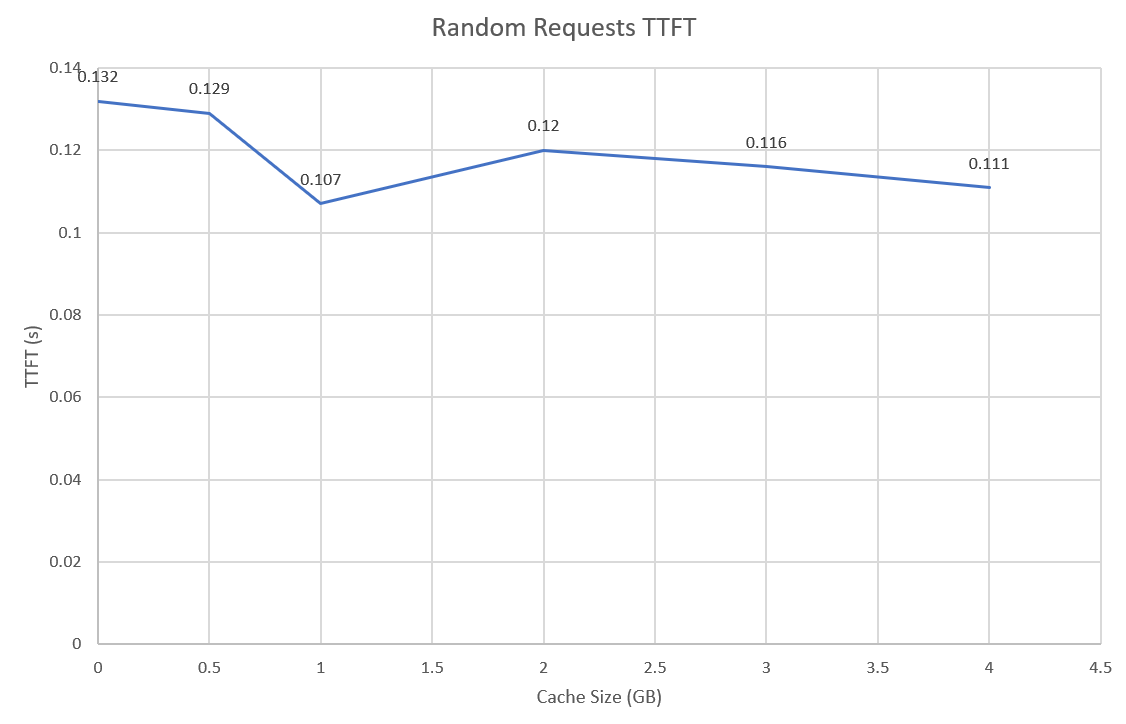
\includegraphics[width=\linewidth]{lmcache-vllm-extended/frontend/results/q3/RandomRequestTTFT.png}
\caption{Random Requests - TTFT}
\end{subfigure}\hfill
\begin{subfigure}{0.48\textwidth}
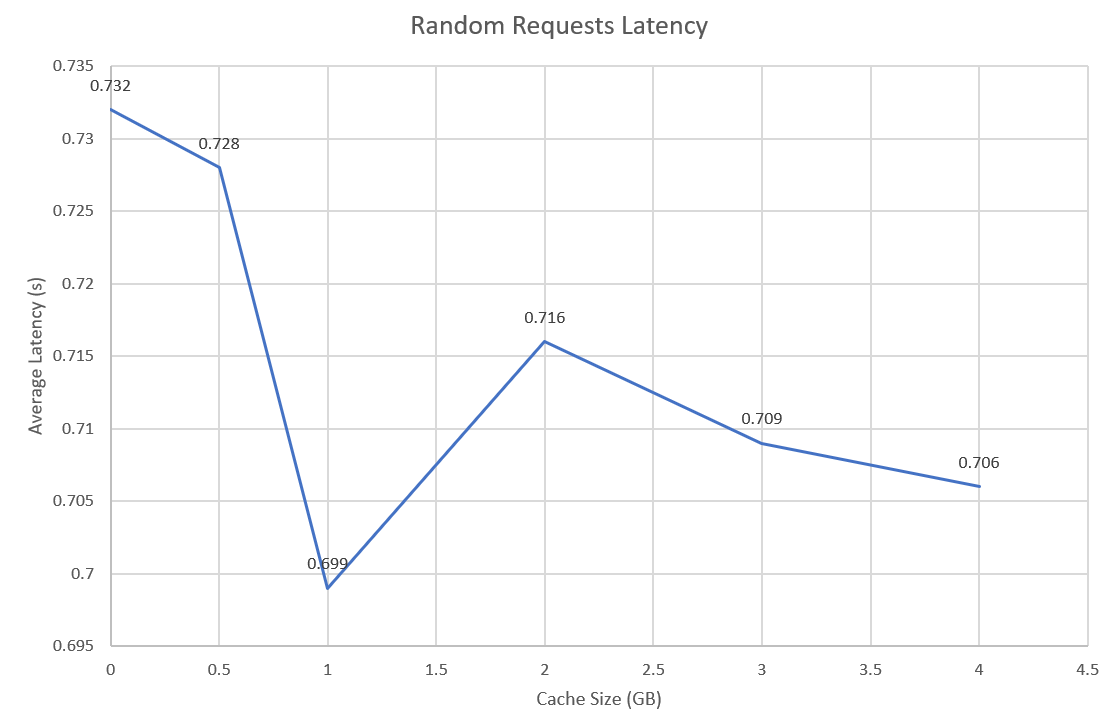
\includegraphics[width=\linewidth]{lmcache-vllm-extended/frontend/results/q3/RandomRequest-Latency.png}
\caption{Random Requests - Latency}
\end{subfigure}

\vspace{0.3cm}
\begin{subfigure}{0.48\textwidth}
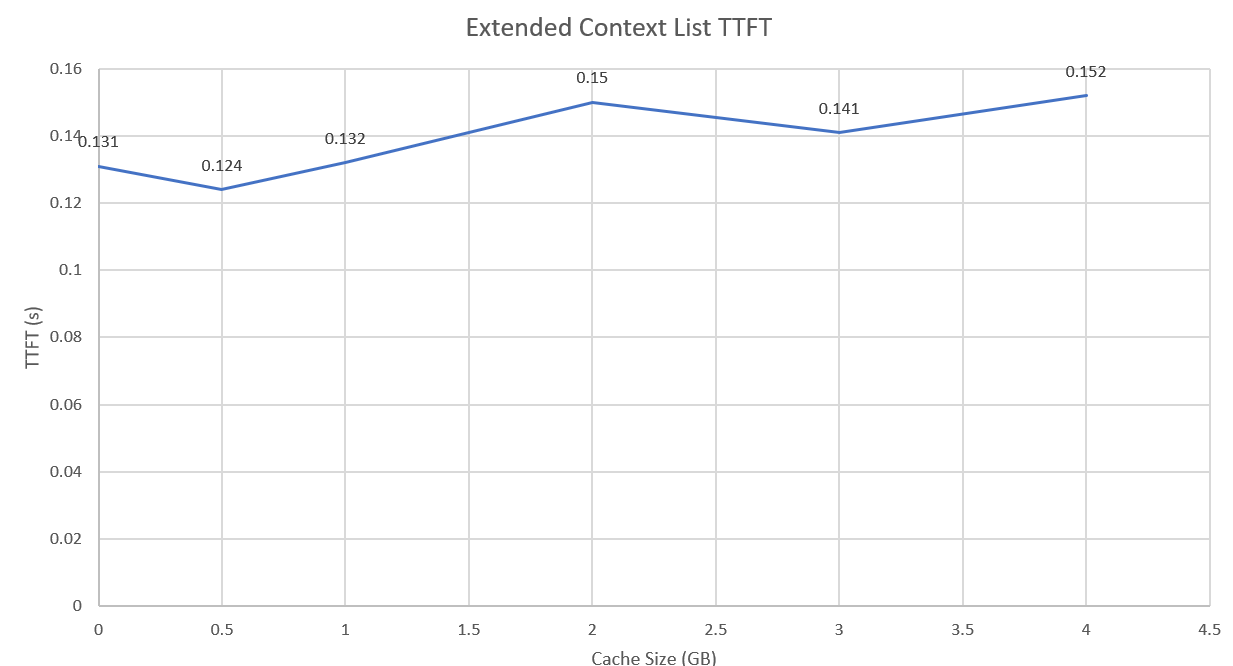
\includegraphics[width=\linewidth]{lmcache-vllm-extended/frontend/results/q3/ExtendedListTTFT.png}
\caption{Extended Context List - TTFT}
\end{subfigure}\hfill
\begin{subfigure}{0.48\textwidth}
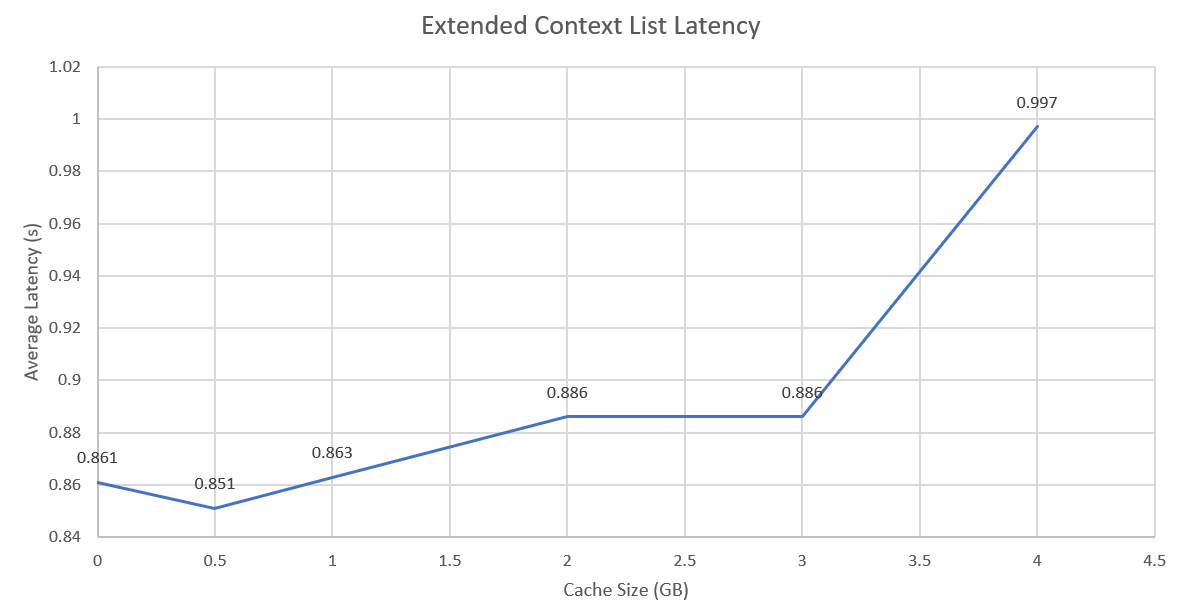
\includegraphics[width=\linewidth]{lmcache-vllm-extended/frontend/results/q3/ExtendedListLatency.png}
\caption{Extended Context List - Latency}
\end{subfigure}
\caption{Results for the TTFT and Latency of testing across differing GPU memory allocations for KV caching}
\label{fig:q2_timelines}
\end{figure}

When we compare the results obtained during our testing with more random request batches, to the less diverse batches used during our latency vs. sequence length analysis, we can see that the request randomness has a slight performance impact. The average TTFT (excluding first requests) seen during the initial tests ranged from .09-.1 seconds, however on more diverse request batches we notice that the TTFT hovers from .11-.13 seconds across different cache sizes. We still observe an effect of the cache size on both the TTFT and the overall latency for random requests, with both noticeably decreasing until hitting an optimal level at 1 GB (.107 seconds for TTFT, and .699 seconds overall latency). Following 1 GB, when raising cache size further we notice a slight spike in both metrics for 2GB, before staying quite level at higher cache sizes. 
\newline\newline
We can also see a similar impact when we analyze the results using an extended and more diverse context list. We see that the TTFT and the overall latency are higher during more random request samples when we provide more contexts for the request batch, with a .13-.15 seconds TTFT, and .85-1 seconds overall latency. This is in constrast to the previously mentioned .11-.13 seconds TTFT and .7-.73 seconds latency when using just our original context list. We also notice the optimal cache size during these runs seems to be slightly less, with the best times achieved at a cache size of just 0.5GB. 
\newline\newline 
These results seem to show that as more diversity gets introduced to the requests served to the LLM, the benefits of a large KV cache size are noticeably diminished. 

\section{Task 2}

\section{Task 3}


\section{Task 4}


\end{document}